\documentclass[a4paper,13pt,twoside]{book}
\usepackage[english]{babel}
\usepackage[utf8]{inputenc}
\usepackage{graphicx}

\pagestyle{headings}
\begin{document}

\chapter{Introduction}

\section{Definition: Object detection}
Object detection is the process of to find a classification for each object on an image.

Classification consists of localisation and labelling an object in an image.
Localisation introduces a bounding box which is used to mark the position of an object in an image.
By processing the image data the system is able to find a class label (Labelling) for the object.

\section{Applications: Object detection}

Object detection has many applications in the industry.

Self driving cars use object classification to detect pedestrians on the streets.
Face recognition systems use object detection to offer a comfortable and secure way to lock smartphones.
Supermarkets use object detection to automatically checkout customers by recognition of products that are taken from the shelves, creating a virtual shopping list and processing payments through smartphones.

\chapter{Convolutional neural networks}

The term 'Convolutional neural networks' is composed of 'Convolution', a set of operations, and 'Neural networks', well-known algorithm of artificial neural networks. Convolutional neural networks are the combination of these two ideas.

Convolutional neural networks break down to feeding an image as input data into the network, learning features and classification. Feature learning applies filters to the image to break up the linearity. This is done by using a rectifier function. The process creates feature maps which are then pooled for further classification. By flattening the pooled feature maps, classifcation outputs the result through the fully connected layer.

Throughout this entire process, the network's building blocks, like the weights and the feature maps, are trained and repeatedly altered in order for the network to reach the optimal performance that will make it able to classify images and objects as accurately as possible.

\section{Image input}

Images can be considered as a matrix of pixels. In order to input this matrix into the convolutional network each pixel is split into its RGB (Red Green Blue) values. The resulting matrixes can be inputted into the network and will be used to stimulate the input neurons.

\{Feature learning}

\section{Convolution}

Neural networks are composed of artificial neurons, which simulate biological neurons in a limited way.

By stimulation from input neurons a convolutional neural network can learn features. Features can be geometric shapes. Low-level-features are basic geometric shapes which are hard to recognise for a human being. High-level-features on the other hand can become more complex like faces, cars or other objects. The complexity is created by the amount of convolutional layers in the network.

In order to convolve a feature, a filter matrix is applied to the processed data. This results in a new matrix which can then be further processed.

A filter in a convolutional layer takes live data as well as predetermined balancing coefficients from the training of the network into account.

The training adds a weight to each connection from a previous neuron and a bias which is independent from the input neurons. By accumulation of all weighted neural inputs and the bias a stimulation can be determined.

To activate following neurons, the network uses activation functions which take the stimulation of the neuron into account and produces an output stimulation to each following neuron.

\section{Activation function}

Neural network activation functions are a crucial component.
Activation functions are mathematical equations that determine the output of a neural network.

The function is attached to each neuron in the network, and determines whether it should be activated or not, based on whether each neuron’s input is relevant for the model’s prediction.

Modern neural networks use a commonly used technique called backpropagation to train the network. The objective of backpropagation is to change the weights for the neurons, in order to bring the error function to a minimum. With this process the model is trained, which places an increased computational strain on the activation function, and its derivative function and to reduce training time. Over time, activation functions have become more performant. There are linear and non-linear types of activation functions. The Linear activation function does not allow backpropagation. That's why they are unpopular. Non-linear activation functions include sigmoid, hyperbolic tangent and (leaky) ReLU.

\section{Sigmoid function}

The sigmoid which has high biological plausibility. It has output values between 0 and 1.

For a value of X above 2 or below -2, tends to bring the Y value (the prediction) to the edge of the curve, very close to 1 or 0. This enables clear predictions.

The smooth gradient of the sigmoid function prevents outliers.

There are also disadvantages in using the sigmoid function.

For very high or very low values of X (input tensor/variable to compute activation function), there is almost no change to the prediction, causing a vanishing gradient problem. This can result in the network refusing to learn further, or being too slow to reach an accurate prediction.

A small gradient means that the weights and biases of the initial layers will not be updated effectively with each training session. Since these initial layers are often crucial for recognizing the core elements of the input data, it can lead to overall inaccuracy of the whole network.

The sigmoid function is computationally expensive.

\section{Hyperbolic tangent}

Hyperbolic tangent is zero centered which balances the amount of positive and negative values. Therefore it is easier to model inputs that have strong negative, neutral, and strong positive values.

It has the same disadvantages as the sigmoid function.

\section{ReLU}

ReLU is more efficient and allows the network to converge very quickly.

ReLU is a non-linear function, although it looks like a linear function. On top of that it has a derivative function and allows for backpropagation.

\section{(Leaky) ReLU}

Other than leaky ReLU there are also other ReLU which is not in use nowadays because it does not provide consistent predictions for negative input values.

\section{Chained convolution}

\begin{figure}[h!]
  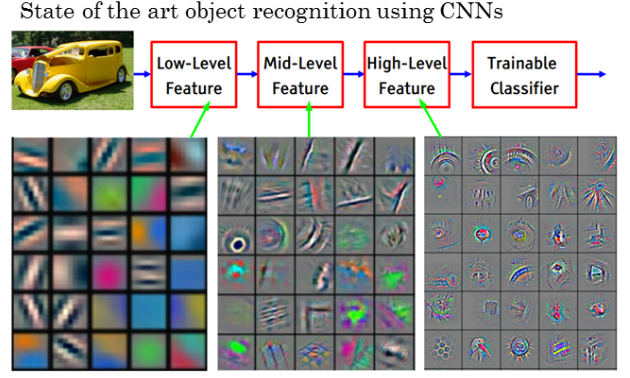
\includegraphics[width=\linewidth]{Images/chainedconvoluion(17).png}
  \caption{Chained Convolution.}
  \label{fig:Chained Convolution}
\end{figure}

Activation function will be used more than once.

The first Convolutional Layer is responsible for capturing the Low-Level features such as edges, color, gradient orientation, etc.

With added layers, the architecture adapts to the Mid-level Feature as well as High-Level features, which provides a network which has the wholesome understanding of images in the dataset.

In the low-level feature the edges, color, gradient are being detected. In Mid-level feature it is more clear to see the form of the objective and in the High-level feature it almost looks like a tyre.

\section{Pooling}

\begin{figure}[h!]
  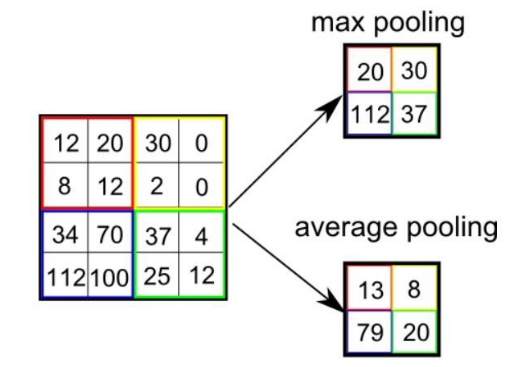
\includegraphics[width=\linewidth]{Images/pooling(18).png}
  \caption{Pooling Layer.}
  \label{fig:Pooling}
\end{figure}

Pooling layers reduce noises in the data and optimise the performance of the network by filtering insignificant data.

Similar to the Convolutional Layer, the Pooling layer is responsible for reducing the size of the Convolved Feature.
The image contains a lot of pixel values and is typically easy for the network to learn the features if the image size is progressively reduced.

Pooling is used to decrease the computational power required to process the data through dimensionality reduction.

There are two types of pooling.

Average Pooling returns the average of all the values from the portion of the image covered by the Kernel.
Average pooling is not used often, but max pooling is used in most of the examples.
Average Pooling simply performs only dimensionality reduction rather than reducing noise.

Max Pooling returns the maximum value from the portion of the image covered by the Kernel.
Max Pooling also reduce noise in data. It discards the noisy activations altogether and also performs de-noising along with dimensionality reduction.
Therefore, we can say that Max Pooling performs a lot better than Average Pooling.

\section{Hidden layer}

\begin{figure}[h!]
  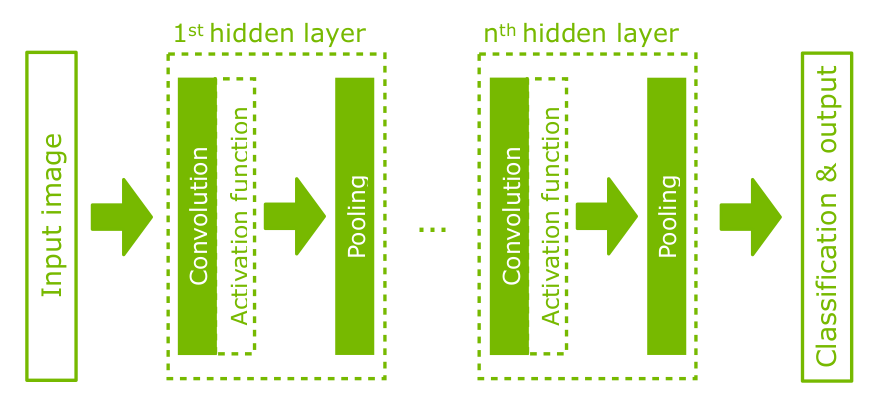
\includegraphics[width=\linewidth]{Images/hiddenlayer(19).png}
  \caption{Hidden Layer.}
  \label{fig:hiddenlayer}
\end{figure}

The Convolutional Layer and the Pooling Layer, together form the n-th layer of a Convolutional Neural Network, which is also known as a Hidden layer.
The amount of hidden layers in a convolutional neural network determine how complex features can become. A network with a large amount of hidden layers can be considered a „Deep Convolutional Neural Network“.

Depending on the complexities of the images, the number of such layers may be increased for capturing low-levels details even further, but at the cost of more computational power.

\section{Classification & output}

After going through the above processes, it enables the model to understand the features. After that the final output matrix from the last pooling layer is then flattened and fed to regular neural network for further classification purposes.

\section{Softmax}

Before the Output Layer a Softmax function is used which is an activation function.

A Softmax function limit the output of the function into the range  0 to 1. This allows the output to be interpreted directly as a probability.

The Softmax layer must have the same number of nodes as the output layer.

\section{Flatten}

\begin{figure}[h!]
  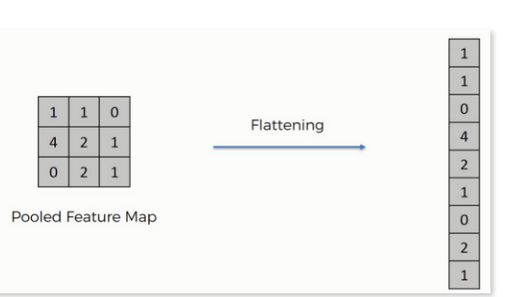
\includegraphics[width=\linewidth]{Images/flatten(22).png}
  \caption{Flatten.}
  \label{fig:flatten}
\end{figure}

Flattening means transforming the output m x n matrix from pooling layer to 1 dimensional column vector.

The first row first column element of the matrix would be the first element of the vector then the next one on the right side would be the second element. And it goes on from left to right row by row till it reaches the last row last column element of the matrix.

\section{Fully connected layer}

\begin{figure}[h!]
  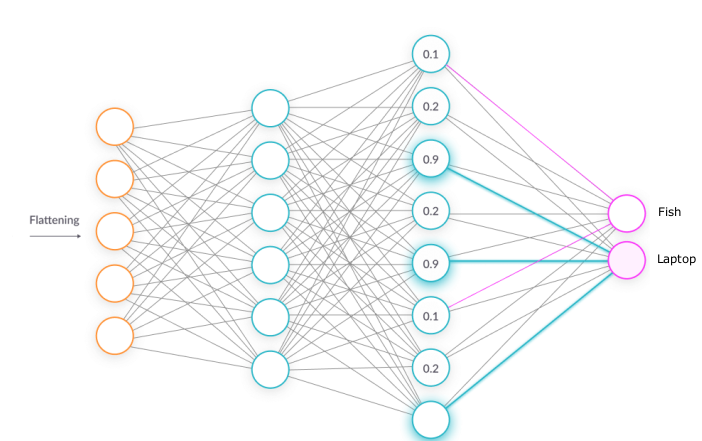
\includegraphics[width=\linewidth]{Images/fullyconnectedlayer(23).png}
  \caption{Fully Connected Layer.}
  \label{fig:fully connected layer}
\end{figure}

The objective of a fully connected layer is to take the results of the convolution/pooling process and use them to classify the image into a label (in a simple classification example).
At the very beginning, we have an input image which we convolve, pool, flatten, and then pass through the artificial neural network.
By the end of this channel, the neural network issues its predictions. For example,the network predicts the figure in the image to be a laptop by a probability of 80%, yet the image actually turns out to be of a fish. An error has to be calculated in this case.

This error is known as Loss Function.

The loss function informs, how accurate the network is, which is then used in optimizing the network in order to increase its effectiveness.

These include the weights (the blue lines connecting the neurons, which are basically the synapses) and the feature detector since the network often turns out to be looking for the wrong features and has to be reviewed multiple times for the sake of optimization.

As the network is optimized, the information keeps flowing back and forth over and over until the network reaches the desired state.

The neuron in the fully-connected layer detects a certain feature, (e.g. a screen as shown in the picture) preserving its value.
It communicates this value to both the “laptop” and the “fish” classes, which checks out the feature and decide whether it's relevant to them or not.

This happens gradually as it receives the same reading multiple times. The laptop class on its part will start focusing more on the attributes carrying the highest weight (the three thick skyblue lines), and it will ignore the rest.

This process keeps repeating until we have an optimized neural network.

The previous layer passes on which of these features it detects, and based on that information, both classes calculate their probabilities, and that is how the predictions are produced.

\chapter{Advanced CNNs}

\section{Bounding box}

\begin{figure}[h!]
  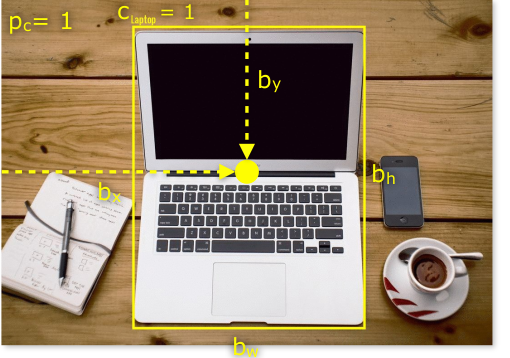
\includegraphics[width=\linewidth]{Images/boundingbox27.png}
  \caption{Bounding Box.}
  \label{fig:Bounding Box}
\end{figure}

In object detection, bounding boxes are used to locate the specific Objects in an image. The bounding box is a rectangular box which can be determined with the help of coordinates:
bx as X-axis and by as Y-axis (in the above picture)
The coordintes begin from the upper left corner of the image.
X-axis is read from upper left to right.
Y-axis is read from top to bottom.
The origin of the coordinates in the image is the upper left corner of the image, and to the right and down are the positive directions of the X-axis and the Y-axis respectively.

\section{Multiple Objects}

\begin{figure}[h!]
  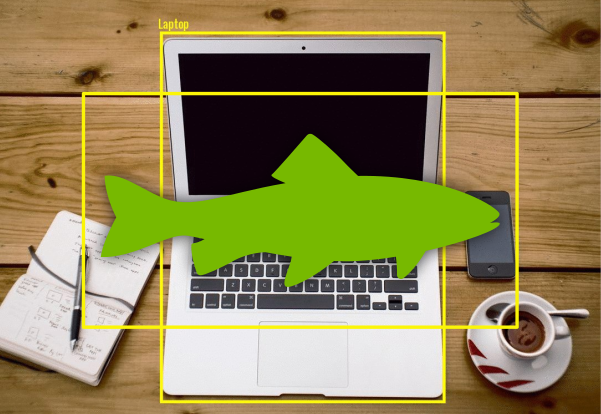
\includegraphics[width=\linewidth]{Images/multipleobjects28.png}
  \caption{Multiple Objects.}
  \label{fig:Multiple Objects}
\end{figure}

An image can contain multiple objects overlapping eachother as shown in the picture (a laptop and a fish), consisting of two bounding boxes, horizontal box focusing the fish and vertical box focusing the laptop.
As a end result, after measuring both the X and Y-axis coordinates for the both bounding boxes, which determines two different objects in a single image where the laptop is partially overlapped by the fish.

\section{Support Vector Machines (SVM)}

Each of the 2000 region proposals generated from every image (using the selective search algorithm) are converted into fixed inputs of size 227 x 227 by a simple warping, irrespective of the size or aspect ratio to enable their use in fine-tuning the CNN (we need fixed-sized inputs irrespective of the actual dimensions to feed to the CNN).
The class-specific dot products between the features and SVM weights are combined into a single matrix-matrix product for an image (Figure ). That is, for every image, a 2000 x 4096 feature matrix is generated (the 4096-d feature from the CNN for all 2000 region proposals). The SVM weight matrix is 4096 x N where N is the number of classes.

\section{Bounding box regression}

\section{Regional Convolutional Neural Network (R-CNN)}

Regional convolutional neural networks are a combination between traditional methods and convolutional neural networks.
Traditional methods are great in recognizing objects within the image, however they do not implement automatic classifers for new objects. In other words, new objects have to be added manually. By combining traditional methods and convolutional neural networks it can outsource the automatic classifer to the convolutional neural networks. Still there is the problem of fixed size images that the convolutional neural networks needs. It is not convenient to only accept one size of images. The solution is a wrapper that simply reduces the size of an image but in execute this wrapper the image often lost is orginal shape.

Unfortunatly, there is a new problem and thats the training due to wrap resizing. To fix that problem, building a complex pipline can be considered as a solution. Objects are represented as a vectors. Each vector has a flag which indicates whether the object is part of the class or not. Usually, traditional methods generate about 2000 potential objects.

The steps required to classify an image are detection of features, generation of feature maps, allocation of features to objects and adaption of the image size to the fully connected layer.

The first step starts with an image whose size does not need to be the fixed, followed by feature localisation which applies traditional methods to extract potential objects. R-CNNs process objects separately. Each object is resized to the fixed size in the wrap region. Both are external, as they are not part of a normal convolutional neural network. Further feature localisation makes use of normal convolutional neural networks.

Feature learning determines characteristics of the object. Flatten layers are used to transform matrix to a vector. The fully Connected layer finds a class label.

SVMs are used for the training of convolutional neural networks. Also traditional methods become adapted.

Bounding box regression is used to improve the boxes. Their shape, size and position become more accurate.

Pros/Cons

Regional convolutional neural networks are simple. Its average training time is about 50 seconds per image. Processing thousands of images takes too long. SVM contains vectors describing objects in an image rather than just a class label. Complex pipelines are used for backpropogation (training).
Fast R-CNNs are inaccurate because of an inefficient training process.

Summary

Regional convolutional neural networks are the simplest solution and thats makes it perfect if u want to build ur first image recognition software without an framework. By using frameworks or going advanced it perfomrs very poorly so no recommendation.

\section{Region of Interest (RoI) pooling}

Region of interest pooling uses pooling layer in a loop to reduce the size of an image until it gets the fixed size required by the fully connected layer.

A triangle like shape can be seen in the above picture. Each pooling layer reduces the size to 1/4 of the orginal size.
This is a better alternative to the wrap layer because it is already used in normal convolutional neural networks where backpropogation is applied. Complex piplines become obsolete.

\section{Fast R-CNN}

Fast regional convolutional neural networks are a combination of R-CNN, RoI-Pooling. Also feature localisation and feature feature learning are reversed. Less data has to be processed by the internal convolutional neural network.

Instead of sending each possible object through the convolutional neural networks, detection and classification of features (including traditional methods) are splitted. Feature learning creates feature maps which apply traditional methods to identify the positions and the number of objects. RoI-Pooling reduces the feature map size to a fixed size vector for the fully connected layers to find a class label. Bounding box regression is used to train the networks capabilities to create bounding boxes. To train the CNN itself the softmax function is used. Fast R-CNNs output probabilities for class labels rather than just a flag.

\section{Region proposal network (RPN)}

Region proposal networks are convolutional neural networks whose only purpose is to recognize objects within a feature map.

Using only one convolutional layer a sliding window is applied to a 3x3 sized part of the input matrix. This creates anchor-boxes in every possible rectangle shape and size within the image. To rescale to a specific size (128px, 256px, 512px, a exponent of 2) an intermediate layers is used.

The classification layer indicates for each box whether it contains an object. That's why people call it 2*k score (k is parameter for the possible box). The training applies bounding box regession to determine whether a box has the right length, width and position x, y.

\section{Faster R-CNN}

Faster R-CNNs use RPN instead of traditional methods (unlike fast R-CNNs) detect features in an image and create bounding boxes on feature maps.

PROS/CONS

With about 0.2s per image it can be trained very fast, while suitable for training in computer clusters. Also it is less prone to errors (detecting unusual shapes more accurate than fast R-CNN).

On the other hand faster R-CNNs are very complex. Therefore it is hard to figure out  errors or a falsely trained network. Sometimes it can be slower than fast R-CNN, espescially when it comes to traning on a single CPU.

The speed and accuarcy boost will be gained by parallel working conditions. This requires special resources. Comparing faster R-CNN to fast R-CNN, there is no increase in performance whether training the network in a small computer network or on a single CPU.

\section{YOLO (You only look once)}

To increase the overall performance of the network even further YOLO uses „grids“ which divides the image into subareas instead of creating every possible box. Less boxes have to be created. This leads to a huge leap in performance. To be even more efficent YOLO uses RPNs and CNNs. Fewer convolutional layers are needed.

On the other hand it becomes more complex and extremely diffcult to understand what exactly is happening. Internally, the network seperates the creation of bounding boxes from computing the confidence.

YOLO projects a grid on the input image (non fixed size). Many cells in a grid increase accuracy and decrease the speed of the network. Simultaneously, CNNs create bounding boxes and classify them. Instead of feature maps, feature learning outputs bounding boxes and a confidence for a feature. Further the results get flattened for the fully connected layer. Classfication finds a label for each object on the grid. Also YOLO determines whether every box acquires an individual class label. In the end YOLO implements bounding box regression and the softmax function.

\section{Non-Max-Suppression}

R-CNN and fast R-CNN have a disadvantage compared to faster R-CNN. To reduce the number of bounding boxes to one the non-max-surpression is used. CNNs trigger the non-max-suppression-function to determine whether another box is overlapped with the same class. If overlapping occurs, only the box with the highest class score is kept while the others are dropped.

\end{document}
